\chapter{Implementação computacional}

A implementação computacional das rotinas desenvolvidas nesta dissertação foi feita em linguagem livre Python, que é gratuita, bem documentada, roda em praticamente todos os sistemas operacionais e vem sendo amplamente utilizada pela comunidade científica.  
As rotinas desenvolvidas ao longo deste trabalho foram baseadas no pacote \textit{Fatiando a Terra} \citet{uieda-proc-scipy-2013}, que é livre, de código aberto e desenvolvido para modelagem e inversão em geofísica. A documentação e as instruções para instalação da versão mais atual do \textit{Fatiando a Terra} podem ser encontrados em http://www.fatiando.org.
As rotinas desenvolvidas aqui estão livremente disponibilizadas no Github pelo link: https://github.com/DiegoTaka/ellipsoid-magnetic.

A Figura \ref{fig:Cookbook_Triaxial} exemplifica como calcular a anomalia de campo total $\Delta T (\mathbf{r})$ (Eq. \ref{eq:delta-T-tilde-approx}) gerada por um elipsoide triaxial.
Como mostrado neste exemplo, é necessário importar outros módulos do \textit{Fatiando a Terra} antes de criar o modelo elipsoidal desejado.
A parte \textit{``The local-geomagnetic field"} define a intensidade ($nT$), inclinação e declinação $(º)$ do campo geomagnético local.
A variável \textit{``model"} contém um objeto da classe \textit{``EllipsoidTriaxial"}, que foi desenvolvida neste trabalho como parte do subpacote \textit{``mesher"} do Fatiando a Terra. Esta variável contém os parâmetros que definem o modelo de elipsoide triaxial. Os parâmetros são, respectivamente: posição $x_c$, $y_c$ e $z_c$ ($m$) do centro do corpo, semi-eixos $a$, $b$ e $c$ ($m$), orientações de \textit{strike, dip e rake} $(º)$ e um dicionário que contém as propriedades físicas do modelo. O item \textit{``remanence"} contém a intensidade ($A/m$), inclinação e declinação $(º)$ do vetor de magnetização remanente $\mathbf{M}_{R}$ (Eq. \ref{eq:M-p-remanence}). O item \textit{`k'} contém as susceptibilidades principais $k1$, $k2$ e $k3$ (Eq. \ref{eq:K}) e as orientações \textit{strike}, \textit{dip} e \textit{rake} utilizadas para calcular os vetores unitários $\mathbf{u}_{1}$, $\mathbf{u}_{2}$ e $\mathbf{u}_{3}$ que formam as colunas da matriz ortogonal $\mathbf{U}$ (Eq. \ref{eq:K}). Os vetores foram calculados utilizando-se as Eqs. \ref{eq:v1_triaxial_prolate},
\ref{eq:v2_triaxial_prolate}, \ref{eq:v3_triaxial_prolate}.
As linhas seguintes definem as coordenadas dos pontos $(x, y, z)$ em que será calculada a anomalia de campo total produzida pelo modelo elipsoidal.
Para tanto, utilizou-se o subpacote \textit{``gridder"} do Fatiando a Terra. Neste exemplos, os pontos estão distribuídos em uma grade regular de 200 x 200 (definida pela variável \textit{``shape"}), sobre um plano horizontal em $z = 0$ m. Os pontos são calculados sobre uma área que varia de -5000 até 5000 metros ao longo das direções $x$ e $y$, tal como definido pela variável \textit{``area"}.
As coordenadas são armazenadas nos \textit{``numpy arrays"}: \textit{``xp", ``yp" e ``zp"}. Em seguida, a anomalia de campo total é calculada utilizando-se a rotina \textit{``tf\underline{ }c"}. Esta função está contida no módulo \textit{``ellipsoid\underline{ }triaxial"}, que foi desenvolvido neste trabalho como parte do subpacote \textit{``gravmag"} do Fatiando a Terra. As linhas finais do exemplo mostrado na Fig. \ref{fig:Cookbook_Triaxial} são para plotar a anomalia de campo total produzida pelo modelo elipsoidal utilizando-se o módulo \textit{``mpl"}, que está contido no subpacote \textit{``vis"} do Fatiando a Terra.

A Fig. \ref{fig:anomaly_exemplo} mostra o resultado produzido pelo código da Fig. \ref{fig:Cookbook_Triaxial}. A Fig. \ref{fig:func_triaxial} mostra o código fonte da rotina \textit{``tf\underline{ }c"} (Fig. \ref{fig:Cookbook_Triaxial}) utilizada para calcular a anomalia de campo total mostrada na Fig. \ref{fig:anomaly_exemplo}.
As rotinas também contam com classes que separam os três tipos de elipsoides tratados neste trabalho.

É importante ressaltar que diversos cálculos são feitos com auxílio de bibliotecas do \textit{Python} como o \textit{Scipy} \citet{scipy}, \textit{Matplotlib} \citet{matplotlib} e do pacote \textit{NumPy} \citet{numpy}.
Uma nota a respeito das funções \textit{scipy.special.ellipkinc} e \textit{scipy.special.ellipeinc} do pacote SciPy para o cálculo das integrais elípticas normais incompletas de Legendre de primeiro e segundo tipo (Eqs. \ref{eq:F-kappa-phi} e \ref{eq:E-kappa-phi}): a variável $\kappa$ das funções $F(\kappa, \phi)$ e $E(\kappa, \phi)$ já deve ser elevada ao quadrado.

Tal como definido anteriormente, a soma dos fatores de desmagnetização deve ser igual à 1 (um), independente do tamanho dos eixos e do tipo de elipsoide. Para verificar esta propriedade, foram gerados 200 elipsoides triaxiais com semi-eixos $a = a_0 +u, \, b = b_0+u$ e $c = c_0+u$, em que $a_0=500$ m, $b_0=100$ m, $c_0=50$ m e $500  \le u \le 30000$ m. A Fig. \ref{fig:teste_n_soma} mostra a soma dos fatores de desmagnetização $\tilde{n}^{\dagger}_{11}$, $\tilde{n}^{\dagger}_{22}$ e $\tilde{n}^{\dagger}_{33}$ calculados pelas Eqs. \ref{eq:n-tilde-dagger-11-triaxial}, \ref{eq:n-tilde-dagger-22-triaxial} e \ref{eq:n-tilde-dagger-33-triaxial} para este conjunto de elipsoides e serve como validação de parte das rotinas apresentadas neste trabalho.

\begin{figure}[hbt!]
	\centering 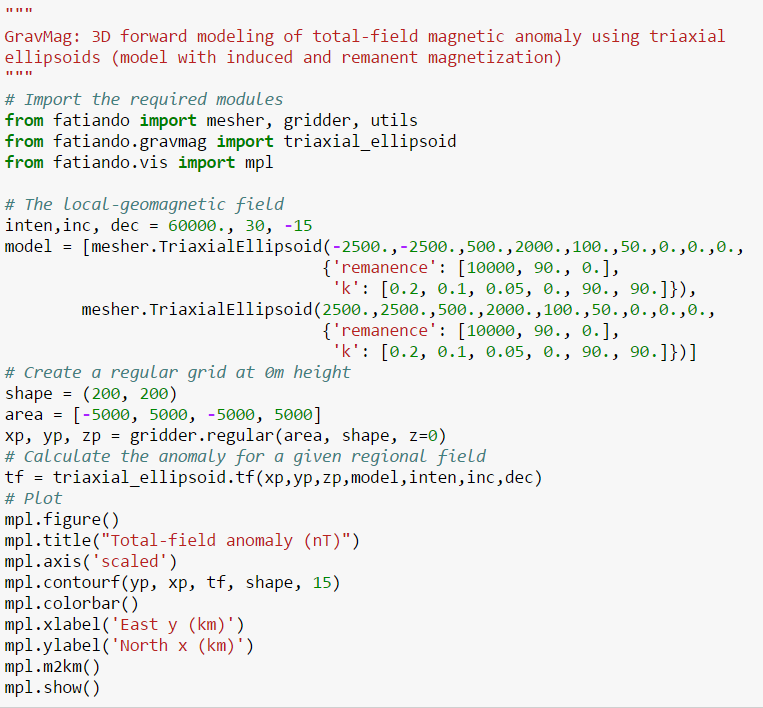
\includegraphics[width=16 cm,height=17 cm]{figures/Cookbook_Triaxial}
	\caption[Exemplo de \textit{script} para gerar um modelo elipsoidal triaxial e calcular a anomalia de campo total $\Delta T (\mathbf{r})$ (Eq. \ref{eq:delta-T-tilde-approx}).]{Exemplo de \textit{script} para gerar um modelo elipsoidal triaxial e calcular a anomalia de campo total $\Delta T (\mathbf{r})$ (Eq. \ref{eq:delta-T-tilde-approx}).}
	\label{fig:Cookbook_Triaxial}
\end{figure}

\begin{figure}[hbt!]
	\centering 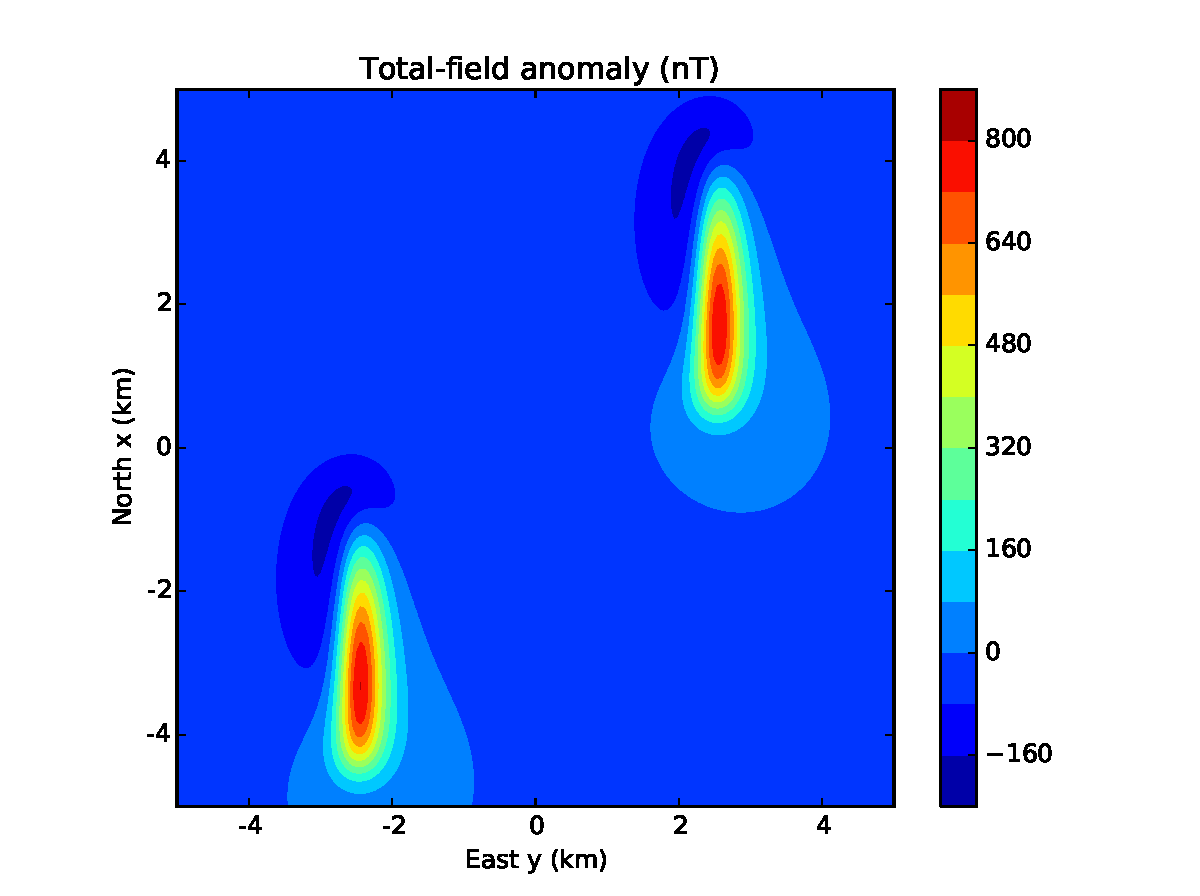
\includegraphics[width=16 cm,height=12 cm]{figures/anomaly_exemplo}
	\caption[Anomalia de campo total $\Delta T (\mathbf{r})$ (Eq. \ref{eq:delta-T-tilde-approx}) produzida pelo código da Fig. \ref{fig:Cookbook_Triaxial}.]{Anomalia de campo total $\Delta T (\mathbf{r})$ (Eq. \ref{eq:delta-T-tilde-approx}) produzida pelo código da Fig. \ref{fig:Cookbook_Triaxial}.}
	\label{fig:anomaly_exemplo}
\end{figure}

\begin{figure}[hbt!]
	\centering 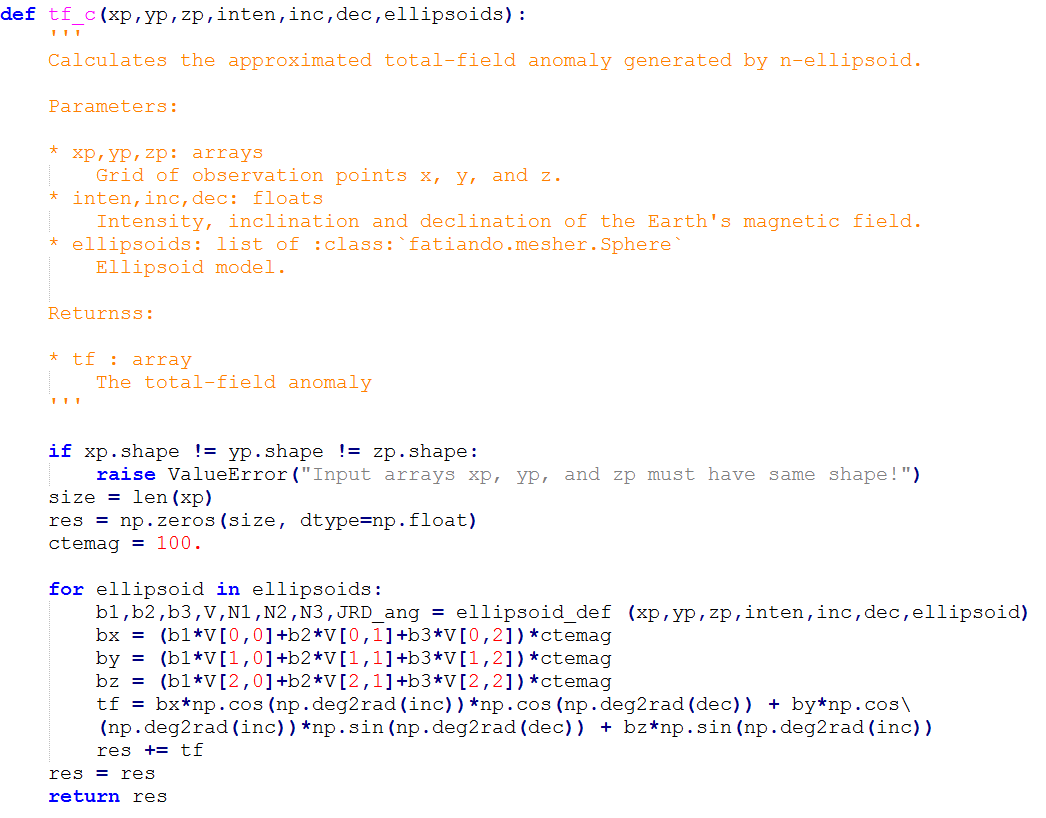
\includegraphics[width=16 cm,height=14 cm]{figures/func_triaxial}
	\caption[Código fonte da rotina \textit{``tf\underline{ }c"} utilizada para calcular a anomalia de campo total $\Delta T (\mathbf{r})$ (Eq.\ref{eq:delta-T-tilde-approx}) produzida pelo modelo elipsoidal definido na Fig. \ref{fig:Cookbook_Triaxial}. Esta rotina utiliza outra rotinas que também foram desenvolvidas neste trabalho como parte do módulo \textit{ellipsoid\underline{ }triaxial} (Fig. \ref{fig:Cookbook_Triaxial}).]{Código fonte da rotina \textit{``tf\underline{ }c"} utilizada para calcular a anomalia de campo total $\Delta T (\mathbf{r})$ (Eq.\ref{eq:delta-T-tilde-approx}) produzida pelo modelo elipsoidal definido na Fig. \ref{fig:Cookbook_Triaxial}. Esta rotina utiliza outra rotinas que também foram desenvolvidas neste trabalho como parte do módulo \textit{ellipsoid\underline{ }triaxial} (Fig. \ref{fig:Cookbook_Triaxial}).}
	\label{fig:func_triaxial}
\end{figure}

\begin{figure}[hbt!]
	\centering 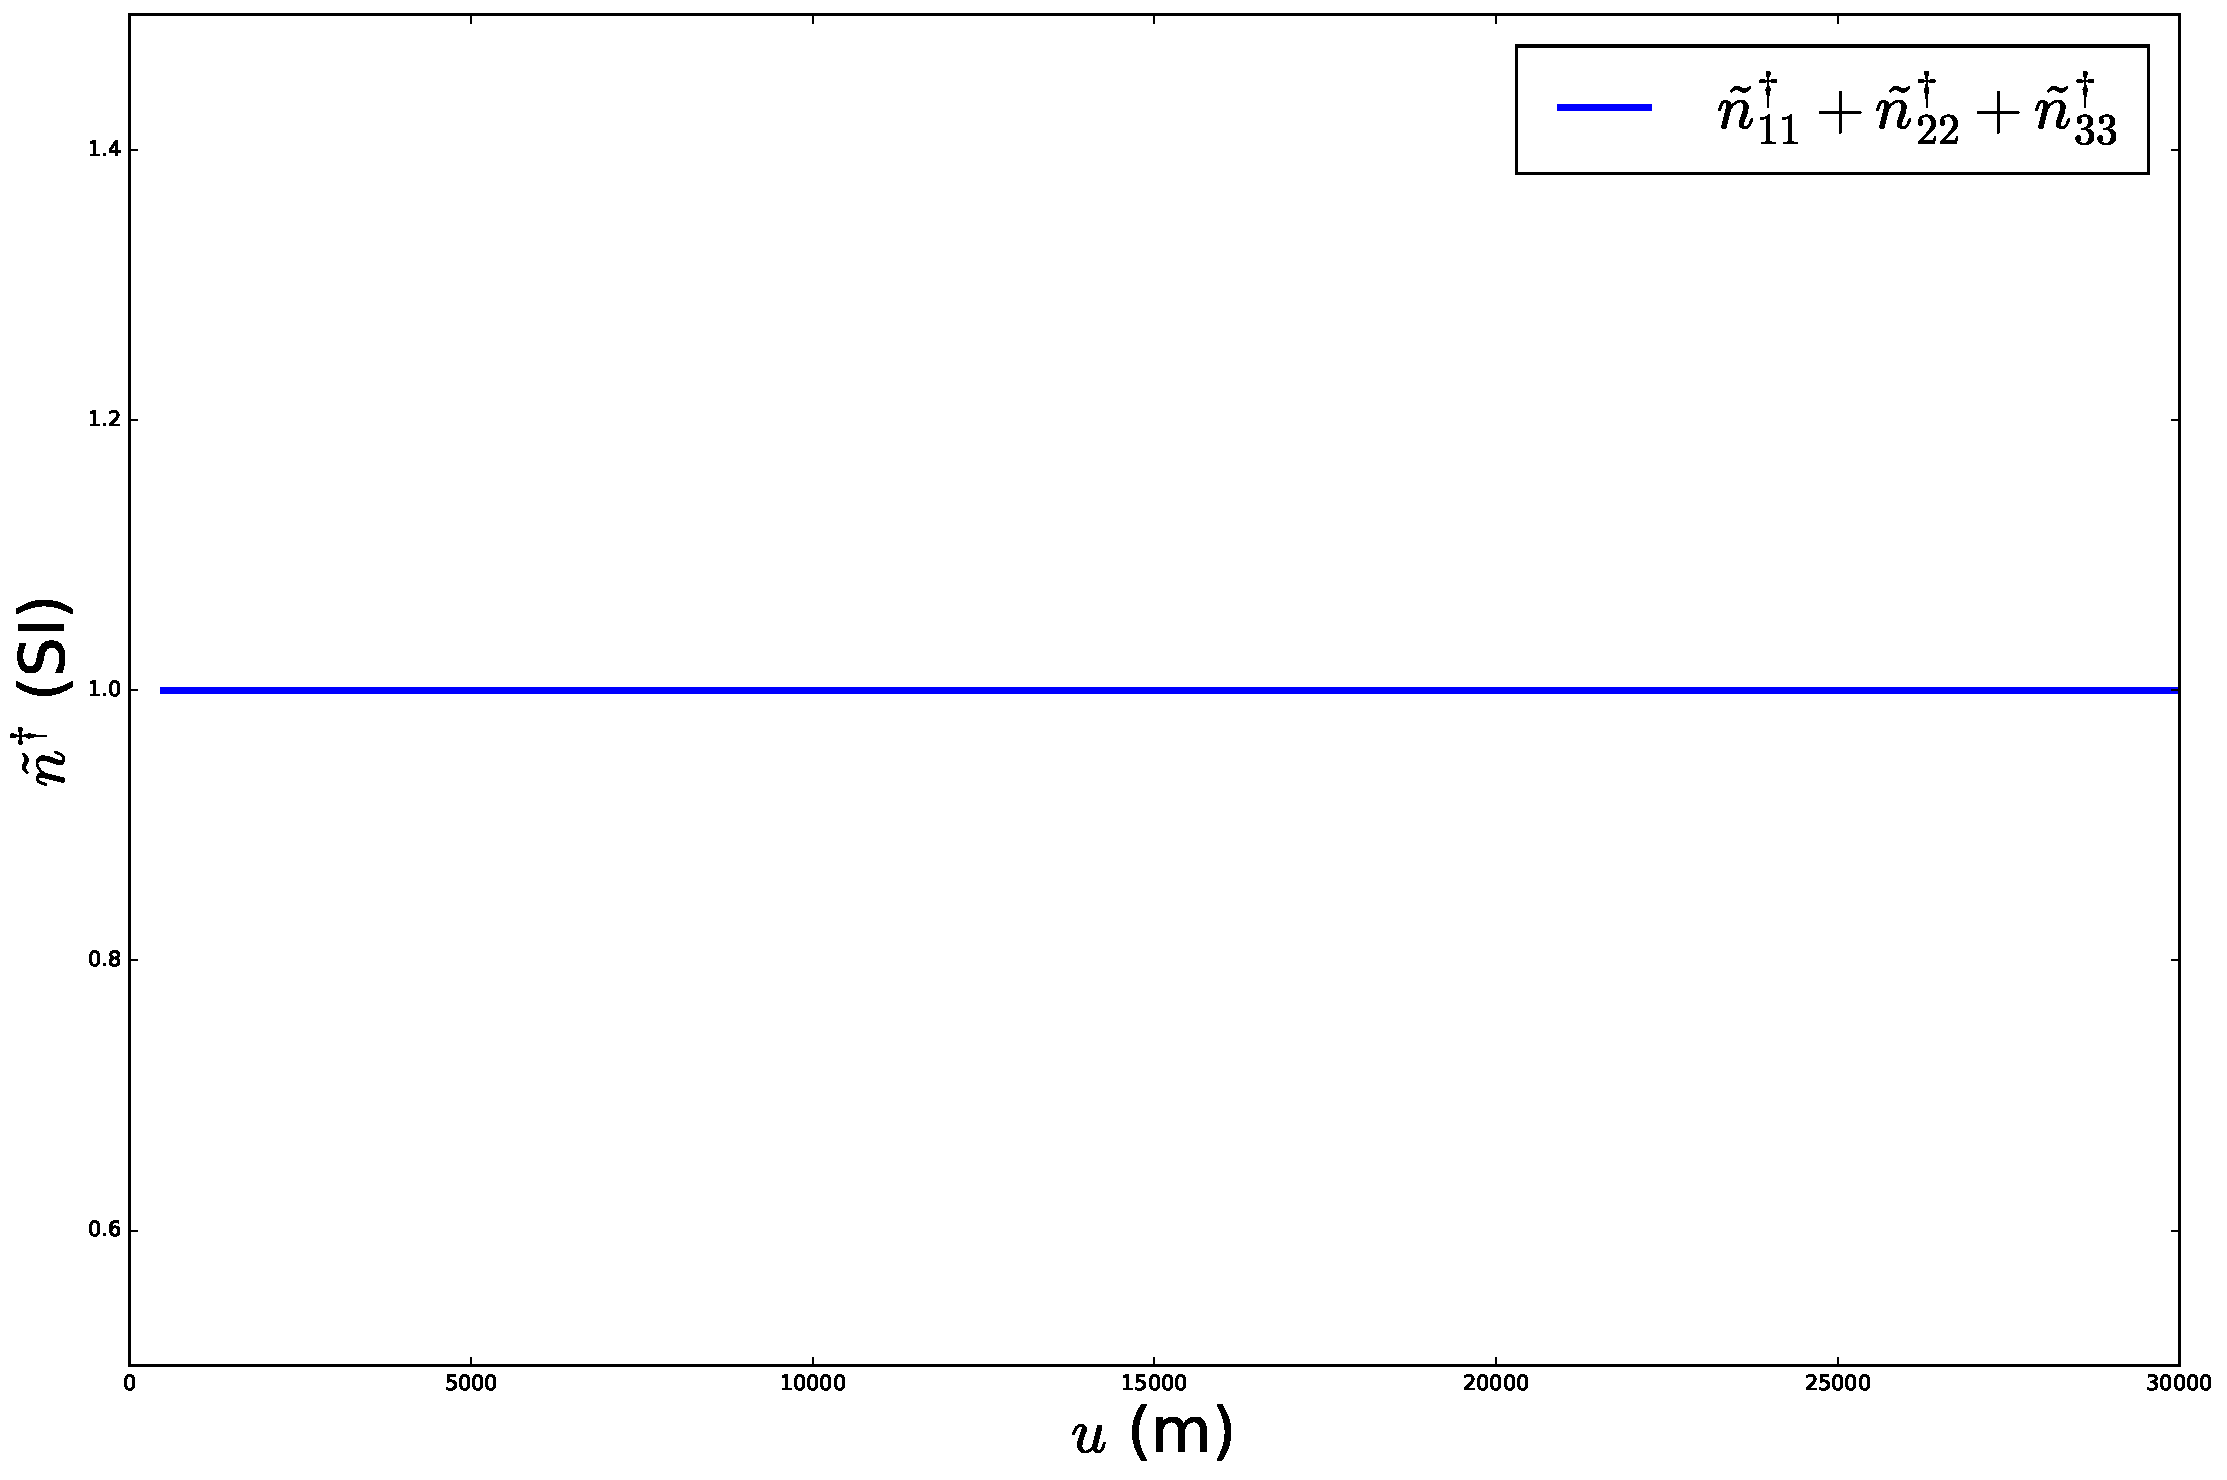
\includegraphics[width=15 cm,height=10 cm]{figures/test_n_soma}
	\caption[Validação dos fatores de desmagnetização. Foram gerados 200 elipsoides triaxiais com semi-eixos $a = a_0 +u, \, b = b_0+u$ e $c = c_0+u$, em que $a_0=500$ m, $b_0=100$ m, $c_0=50$ m e $500  \le u \le 30000$ m. A figura mostra a soma dos fatores de desmagnetização $\tilde{n}^{\dagger}_{11}$, $\tilde{n}^{\dagger}_{22}$ e $\tilde{n}^{\dagger}_{33}$ (Eqs. \ref{eq:n-tilde-dagger-11-triaxial}, \ref{eq:n-tilde-dagger-22-triaxial} e \ref{eq:n-tilde-dagger-33-triaxial}), que está representada pela linha azul, que é igual à 1 (um), independente do tamanho dos eixos e do tipo de elipsoide.]{Validação dos fatores de desmagnetização. Foram gerados 200 elipsoides triaxiais com semi-eixos $a = a_0 +u, \, b = b_0+u$ e $c = c_0+u$, em que $a_0=500$ m, $b_0=100$ m, $c_0=50$ m e $500  \le u \le 30000$ m. A figura mostra a soma dos fatores de desmagnetização $\tilde{n}^{\dagger}_{11}$, $\tilde{n}^{\dagger}_{22}$ e $\tilde{n}^{\dagger}_{33}$ (Eqs. \ref{eq:n-tilde-dagger-11-triaxial}, \ref{eq:n-tilde-dagger-22-triaxial} e \ref{eq:n-tilde-dagger-33-triaxial}), que está representada pela linha azul, que é igual à 1 (um), independente do tamanho dos eixos e do tipo de elipsoide.}
	\label{fig:teste_n_soma}
\end{figure}
